\documentclass[tikz,border=5mm]{standalone}
\usepackage{tikz}
\usetikzlibrary{calc,arrows.meta,decorations.pathreplacing}

\begin{document}

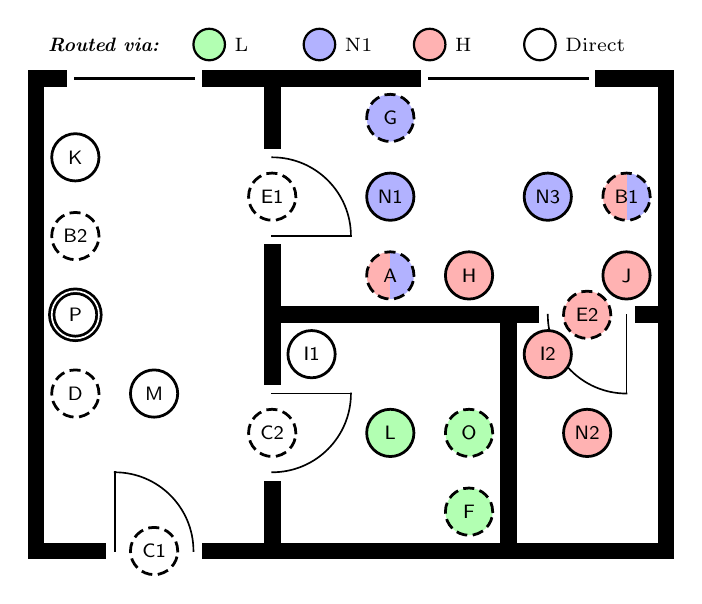
\begin{tikzpicture}[
    x=1cm,y=1cm, % 1 cm = 1 m
    line cap=rect,
    wall/.style={line width=6pt},
    opening/.style={line width=6pt, draw=white},
    thinmark/.style={line width=0.6pt},
    dimarr/.style={-{Latex[length=3mm]}, line width=0.6pt},
    windowline/.style={line width=1pt},
    devmark/.style={circle, draw, fill=white, minimum size=6mm, inner sep=0pt, line width=1pt,
                    font=\scriptsize\sffamily},
    devmark_double/.style={circle, draw, double, fill=white, minimum size=6mm, inner sep=0pt, line width=1pt,
                    font=\scriptsize\sffamily},
    devmark_dash/.style={circle, draw, dashed, fill=white, minimum size=6mm, inner sep=0pt, line width=1pt,
                    font=\scriptsize\sffamily},
]

\tikzset{
  devmark_split/.style 2 args={
    circle, draw, dashed,
    minimum size=6mm, inner sep=0pt, line width=1pt,
    font=\scriptsize\sffamily,
    path picture={
      % Left half: from SW to (x=center, y=max)
      \path[fill=#1, draw=none]
        (path picture bounding box.south west) rectangle
        (path picture bounding box.center |- path picture bounding box.north east);
      % Right half: from (x=center, y=min) to NE
      \path[fill=#2, draw=none]
        (path picture bounding box.center |- path picture bounding box.south west) rectangle
        (path picture bounding box.north east);
    }
  }
}

% --- Basic geometry and parameters ---
\def\W{8}   % width  in meters
\def\H{6}   % height in meters

% --- OUTER WALLS (draw first) ---
\draw[wall] (0,0) -- (\W,0) -- (\W,\H) -- (0,\H) -- cycle;

% --- OPENINGS IN OUTER WALLS (erase segments to create gaps) ---
% Entrance door (bottom wall): from x=1 to x=2
\draw[opening] (1,0) -- (2,0);

% Windows on outer walls
% Top-left (living): x=0.5 to 2.0 on y=H
\draw[opening] (0.5,\H) -- (2.0,\H);
% Top-right (bedroom): x=5.0 to 7.0 on y=H
\draw[opening] (5.0,\H) -- (7.0,\H);

% \draw[opening] (4.0,\W) -- (8.0,\W);
% Bottom (kitchen): x=3.6 to 4.8 on y=0
% \draw[opening] (3.6,0) -- (4.8,0);

% Window detail lines across the gap
\foreach \xa/\xb/\y in {0.5/2.0/\H, 5.0/7.0/\H, 3.6/4.8/0} {
  \draw[windowline] (\xa,\y) -- (\xb,\y);
  \draw[windowline] (\xa,\y) ++(0,0.25);
  \draw[windowline] (\xb,\y) ++(0,0.25);
}

% --- INNER WALLS ---
\draw[wall] (3,0) -- (3,\H);          % main vertical
\draw[wall] (3,3) -- (\W,3);          % horizontal
\draw[wall] (6,0) -- (6,3);           % vertical (kitchen/bath split)

% --- INTERIOR DOOR OPENINGS + swings ---
% Living -> Kitchen
\draw[opening] (3,1) -- (3,2);
\draw[thinmark] (3,2) -- (4,2);
\draw[thinmark] (3,1) arc[start angle=-90, end angle=0, radius=1];

% Living -> Bedroom
\draw[opening] (3,4) -- (3,5);
\draw[thinmark] (3,4) -- (4,4);
\draw[thinmark] (3,5) arc[start angle=90, end angle=0, radius=1];

% Kitchen -> Bathroom
\draw[opening] (6.5,3) -- (7.5,3);
\draw[thinmark] (7.5,3) -- (7.5,2);
\draw[thinmark] (6.5,3) arc[start angle=0, end angle=90, radius=-1];

% Entrance door swing
\draw[thinmark] (1,0) -- (1,1);
\draw[thinmark] (2,0) arc[start angle=0, end angle=90, radius=1];


% % Kitchen -> Bathroom
% \draw[opening] (0,3) -- (0,5);
% \draw[thinmark] (0,3) -- (0,5);
% % =========================================================
% DEVICE MARKERS (circled letters only; non-overlapping)
% =========================================================

% --- Living / Hall (x: 0..3, y: 3..6) ---

\node[devmark_double] at (.5,3) {P};  % Coordinator

  \node[devmark_dash] at (3,4.5) {E1}; % Aqara Door 1
  \node[devmark_dash] at (3,1.5) {C2}; % Sonoff Door 2
  \node[devmark] at (.5,5) {K}; % Ledvance Smart+ Plug
  \node[devmark_dash] at (.5,2) {D};  % Aqara Motion
  \node[devmark_dash] at (1.5,0) {C1}; % Sonoff Door 1
  \node[devmark] at (1.5,2) {M}; % Mose Bulb
  \node[devmark_dash] at (.5,4) {B2}; % Sonoff Motion 2

  \node[devmark,fill=green!30] at (4.5,1.5) {L};  % Ledvance Bulb
    \node[devmark_dash,fill=green!30] at (5.5,1.5) {O};  % Philips Motion
    \node[devmark_dash,fill=green!30] at (5.5,.5) {F};  % Aqara Vibration
    \node[devmark,fill=blue!30] at (4.5,4.5) {N1}; % Philips Lamp 1
      \node[devmark,fill=blue!30] at (6.5,4.5) {N3}; % Philips Lamp 3
      \node[devmark_dash,fill=blue!30] at (4.5,5.5) {G};  % Aqara Button
      \node[devmark_split={red!30}{blue!30}] at (4.5,3.5) {A};  % Sonoff Temperature

  \node[devmark] at (3.5,2.5) {I1}; % Power Plug 1


    \node[devmark,fill=red!30] at (7,1.5) {N2}; % Philips Lamp 2
    

    \node[devmark,fill=red!30] at (5.5,3.5) {H}; % Smart Socket
      \node[devmark_dash,fill=red!30] at (7,3) {E2}; % Aqara Door 2
      \node[devmark,fill=red!30] at (7.5,3.5) {J}; % Ledvance Plug Z3
      \node[devmark,fill=red!30] at (6.5,2.5) {I2}; % Power Plug 2
     
\node[devmark_split={red!30}{blue!30}] at (7.5,4.5) {B1}; % Sonoff Motion 1





\begin{scope}[yshift=-1cm]
  % Reference bottom of main drawing
  \coordinate (legendcenter) at (current bounding box.south);

  % Place the legend below and centered
  \begin{scope}[shift={(legendcenter)}, yshift=7.2cm]
    \tikzset{
      legendline/.style={line width=0.8pt},
      legendtext/.style={font=\scriptsize, anchor=west}
    }


    \def\ycc{-0.45}        % y position of the color-code row
    \def\xccstart{-1.8}  % shifted right to make room for header
    \def\xccstep{1.4}    % horizontal spacing between entries
    
    % Header
    \node[legendtext, anchor=east] at (-2.3,\ycc) {\textbf{\textit{Routed via:}}};
    
    \foreach \i/\col/\lab in {
      0/green!30/L,
      1/blue!30/N1,
      2/red!30/H,
      3/white/Direct
    }{
      \node[circle, draw, fill=\col, minimum size=4mm, inner sep=0pt, line width=0.8pt]
        at ({\xccstart+\i*\xccstep},\ycc) {};
      \node[legendtext]
        at ({\xccstart+\i*\xccstep+0.20},\ycc) {\lab};
    }
    
  \end{scope}
\end{scope}

% \begin{scope}[yshift=-1cm]
%   % Reference bottom of main drawing
%   \coordinate (legendcenter) at (current bounding box.south);

%   % Place the legend below and centered
%   \begin{scope}[shift={(legendcenter)}, yshift=-0.4cm]
%     \tikzset{
%       legendline/.style={line width=0.8pt},
%       legendtext/.style={font=\scriptsize, anchor=west}
%     }

%     % PANC (double line)
%     \draw[legendline, double] (-3.0,0) -- (-2.4,0);
%     \node[legendtext] at (-2.25,0) {PANC};

%     % FFD (solid line)
%     \draw[legendline] (-0.3,0) -- (0.3,0);
%     \node[legendtext] at (0.45,0) {FFD};

%     % RFD (dashed line)
%     \draw[legendline, dashed] (2.4,0) -- (3.0,0);
%     \node[legendtext] at (3.15,0) {RFD};
%   \end{scope}
% \end{scope}








% \node[devmark] at (2.85,4.1) {I2};  % Aqara Door 2 (Living->Bedroom) - inside living

% % --- Kitchen (x: 3..6, y: 0..3) ---
  % Moes Bulb


% % --- Bathroom (x: 6..8, y: 0..3) ---
% \node[devmark] at (6.2,1.5) {I1}; % Aqara Door 1 (Kitchen->Bath) - just inside bath
% \node[devmark] at (7.4,1.0) {J};  % Aqara Vibration

% % --- Bedroom (x: 3..8, y: 3..6) ---

% \node[devmark] at (7.0,4.4) {A3}; % Philips Lamp 3 (near top window)
% \node[devmark] at (7.4,3.4) {H2}; % Power Plug 2

% \node[devmark] at (7.4,5.6) {G};  % Philips Motion
% \node[devmark] at (6.6,5.8) {E2}; % Sonoff Door 2 (top wall opening) - inside bedroom

\end{tikzpicture}
\end{document}